\section{Ашигласан технологиуд, программчлалын хэл}
\subsection{WebRTC}
\footnote{WebRTC official site \url{https://webrtc.org/}}
	\quad \quad WebRTC (Web Real-Time Communication) нь энгийн хэрэглээний программчлалын интерфейс (API) ашиглан веб хөтчүүд, гар утасны программууд болон IoT төхөөрөмжүүдийн хооронд шууд бодит цагийн харилцаа холбоог бий болгох нээлттэй төсөл юм. Энэ нь веб хуудаснууд дотор дуудлага хийх, видео чат хийх, PC хооронд файл хуваалцах боломжийг олгодог. WebRTC-ийн онцлогууд:

	1. Peer-to-Peer Communication: WebRTC нь хөтчүүд болон бусад программуудын хооронд зуучлагч сервер ашиглахгүйгээр бодит цагийн харилцааг идэвхжүүлдэг.
	
	2. Media Streams: PC хооронд аудио болон видео дамжуулах боломжийг олгодог.
	
	3. Өгөгдлийн суваг: PC хооронд дур зоргоороо өгөгдөл дамжуулах боломжийг олгодог.
	
	4. Дохио өгөх: WebRTC нь сигнал тодорхойлж өгөөгүй байдаг. Энэ нь холболтын хяналтын мессежийг солилцоход дохио өгөх сервер шаарддаг боловч сонгох  эсэх нь хөгжүүлэгчээс хамаарна. Websockets, HTTP, XMPP (Extensible Messaging and Presence Protocol) ашиглаж болно.
	
	5. NAT дамжуулалт ба галт ханын зохицуулалт: WebRTC нь NAT дамжуулалтын механизмуудыг агуулдаг бөгөөд энэ нь хоёулаа галт хана эсвэл чиглүүлэгчийн ард байх үед интернэт  дэх үйлчлүүлэгчдийн хооронд өгөгдөл солилцох боломжийг олгодог.
	
	6. Аюулгүй байдал: WebRTC нь нууцлал, аюулгүй байдлын үүднээс Datagram Transport Layer Security (DTLS) болон Secure Real-time Transport Protocol (SRTP) ашиглан медиа урсгалыг шифрлэдэг.
	
	7. Платформ хоорондын нийцтэй байдал: Энэ нь Chrome, Firefox, Safari, Edge, Opera зэрэг томоохон веб хөтчүүдтэй нийцдэг.
	
	8. Нээлттэй эх сурвалж: Нээлттэй төсөл учраас WebRTC нь чөлөөтэй ашиглах боломжтой бөгөөд хөгжүүлэгчдийн өргөн хүрээний дэмжлэгтэй.
	
	WebRTC-ийн программууд нь видео хурал, онлайн тоглоом, файл дамжуулах гэх мэт. Энэ нь веб хуудаснууд болон программууд руу шууд бодит цагийн харилцаа холбоог бий болгох хүчирхэг хэрэгсэл юм.
	\pagebreak
\subsection{Go language}
	\footnote{Go language official site \url{https://go.dev/}}
		\quad \quad Golang гэж нэрлэдэг Go нь Google-ийн боловсруулсан нээлттэй программчлалын хэл юм. Үүнийг Роберт Гриземер, Роб Пайк, Кен Томпсон нар бүтээсэн бөгөөд 2009 онд анх худалдаанд гарсан. Олон цөмт, сүлжээнд холбогдсон машинууд болон том кодын баазуудын эрин үед программчлалын бүтээмжийг сайжруулах зорилгоор уг хэлийг бүтээжээ. Go хэлний гол онцлогууд:

		1. Concurrent and Concurrent: Go нь олон цөмт болон сүлжээнд холбогдсон машинуудаас хамгийн ашигтай программ бичихэд хялбар болгох зорилготой юм. Энэ нь статик хэлбэрээр бичигдсэн, эмхэтгэсэн хэл бөгөөд C хэлнээс салангид бичилттэй боловч санах ойн аюулгүй байдал, санах ойн хог цуглуулах, бүтцийн онцлог, CSP маягийн юм.
		
		2. Энгийн: Энгийн, товч бичилттэй тул унших, бичихэд хялбар болгодог. Энэ нь шаардлагагүй синтакс арилгаж, хөгжүүлэгчдэд программынхаа логик дээр анхаарлаа төвлөрүүлэх боломжийг олгодог.
		
		3. Зэрэгцээ: Goroutines нь Go-ийн ажиллах хугацаанд удирддаг хөнгөн утаснууд бөгөөд хялбар параллель программчлал хийх боломжийг олгодог. Сувгууд нь Goroutines хоорондын харилцаа холбоо, синхрончлохыг хөнгөвчилдөг.
		
		4. Баялаг стандарт сан: Сүлжээ, Cryptography, файлын оролт гаралт гэх мэт төрөл бүрийн ажлуудад иж бүрэн дэмжлэг үзүүлэх баялаг стандарт сантай.
		
		5. Статик бичилт: Статик хэлбэрээр бичигдсэн, өөрөөр хэлбэл хувьсагчийн төрлүүд эмхэтгэх үед тодорхойлогддог бөгөөд энэ нь хөгжүүлэлтийн явцад алдаа гаргахад хялбар засна.
		
		6. Санах ойн хог: Автоматаар санах ойн хог цуглуулдаг бөгөөд энэ нь санах ойг автоматаар удирдаж, санах ойн алдагдал гэх мэт программчлалын нийтлэг алдаанаас сэргийлдэг.
		
		7. Compiled хэл: Mашин кодыг хөрвүүлдэг. Энэ нь Go программыг interpreted хэлээс илүү хурдан болгодог.
		
		8. Cross-Platform: Windows, macOS, Linux зэрэг олон платформ дээр эмхэтгэлийг дэмждэг тул платформ хоорондын программуудыг хөгжүүлэхэд хялбар болгодог.
		
		9. Нээлттэй эх: Нээлттэй эх хэл бөгөөд түүний хөгжлийг хөгжүүлэгчид болон хувь нэмэр оруулагчдын томоохон нөлөөтэй.
		
		10. Google-ээр дэмжигдсэн: Go-г Google хөгжүүлсэн бөгөөд үүнийг Google-ийн олон төсөлд ашиглаж байна. Энэ нь найдвартай байдлыг нэмэгдүүлж, байнгын хөгжил, дэмжлэгийг баталгаажуулдаг.
		
		Go нь веб сервер, сүлжээний хэрэгсэл, тархсан систем болон бусад олон зүйлийг хөгжүүлэхэд түгээмэл байдаг. Энгийн байдал, гүйцэтгэл, зэрэгцээ ажиллахад зориулсан суурилуулсан дэмжлэг нь үүнийг олон хөгжүүлэгчдэд, ялангуяа үүлэн тооцоолол болон микро үйлчилгээний архитектурт сонирхолтой сонголт болгодог.
	\pagebreak
\subsection{TypeScript}
		\footnote{TypeScript official site \url{https://www.typescriptlang.org/}}
			\quad \quad TypeScript нь Microsoft-оос хөгжүүлж, засвар үйлчилгээ хийдэг нээлттэй программчлалын хэл юм. Энэ нь JavaScript-ийн багц бөгөөд ямар ч JavaScript код нь мөн TypeScript кодыг дэмждэг гэсэн үг юм. TypeScript нь хөрвүүлэх явцад программчлалын алдааг олж, урьдчилан сэргийлэхэд ашиглаж болох статик хэл. TypeScript-ийн гол онцлогууд:

			1. Статик бичилт: Хөгжүүлэгчдэд хувьсагчийн төрлүүд, функцийн параметрүүд болон буцаах утгуудыг тодорхойлох боломжийг олгодог. Энэ нь алдааг боловсруулах явцад эрт илрүүлж, кодыг урьдчилан таамаглах боломжтой, өөрөө алдаагаа олоход тусална.
			
			2. Type Inference: Tөрлүүдийг тодорхой заагаагүй тохиолдолд төрлүүдийн тодорхойлолтыг ашигладаг. TypeScript нь хувьсагчийн төрлийг хэрэглээнээс нь тодорхойлох боломжтой байдаг тул төрлийг үргэлж тодорхой тэмдэглэх шаардлагагүй гэсэн үг.
			
			3. Объект хандалтат программчлал: TypeScript нь анги, интерфейс, удамшил, хандалтын хувиргагч (нийтийн, хувийн, хамгаалагдсан), ерөнхий шинж чанарууд зэрэг объект хандалтат программчлалын функцийг дэмждэг.
			
			4. ES6/ES7-ийн онцлог: TypeScript нь ECMAScript 6 (ES6) болон ECMAScript 7 (ES7)-ийн олон функцийг дэмждэг бөгөөд энэ нь орчин үеийн, онцлог шинж чанартай хэл юм. Эдгээр функцүүд нь arrow функцүүд, ангиуд, асинхрончлол/хүлээлт гэх мэт.
			
			5. Tool support: TypeScript нь Visual Studio Code, Sublime Text, WebStorm зэрэг алдартай код засварлагчтай нэгтгэх зэрэг багаж хэрэгслийн хүчтэй дэмжлэгтэй. Редакторууд код бөглөх, дахин боловсруулах, шугаман баримтжуулалт гэх мэт функцийг хангаж чадна.
			
			6. JavaScript сантай нийцтэй: JavaScript санг ашиглах боломжтой. TypeScript тодорхойлолтын файлууд (`.d.ts` өргөтгөлтэй) нь одоо байгаа JavaScript кодын хэлбэрийг дүрсэлнэ.
			
			7. Код засвар: Статик бичих замаар TypeScript нь кодын баазыг ялангуяа том төслүүдэд илүү засвартай болгодог. Энэ нь кодыг баримтжуулахад тусалж, шинэ хөгжүүлэгчдэд ойлгох, хувь нэмэр оруулахад хялбар болгодог.
			
			8. Эмхэтгэх: TypeScript кодыг JavaScript код руу хөрвүүлэх ба дараа нь ямар ч JavaScript орчинд ажиллуулах боломжтой. TypeScript нь төрөл бүрийн зорилтот орчин болон ECMAScript хувилбаруудыг дэмждэг бөгөөд хөгжүүлэгчид хуучин платформуудыг дэмжихийн зэрэгцээ орчин үеийн JavaScript бичих боломжийг олгодог.
			
			9. Support: TypeScript нь өргөн цар хүрээтэй, идэвхтэй нийгэмлэгтэй бөгөөд Microsoft-оос байнгын хөгжүүлэлт, дэмжлэг үзүүлдэг.
			
			10. Нээлттэй эх сурвалж: TypeScript нь нээлттэй эхийн төсөл бөгөөд үнэ төлбөргүй ашиглах боломжтой бөгөөд хэн ч үүнийг хөгжүүлэхэд хувь нэмрээ оруулах боломжтой.
			
			TypeScript нь том хэмжээний веб хөгжүүлэлт, ялангуяа JavaScript-ийг удаан хугацаанд хадгалахаар төлөвлөж буй төслүүдэд ихэвчлэн ашиглагддаг. JavaScript-ийн орчин үеийн шинж чанаруудын хамт статик бичих чадвар нь үүнийг өргөтгөх боломжтой, засвар үйлчилгээ хийх боломжтой программуудыг бүтээх хүчирхэг хэл болгодог. 
	\pagebreak
\subsection{Docker}
		\footnote{Docker official site \url{https://www.docker.com/get-started/}}
			\quad \quad Docker бол контейнер ашиглан программуудыг үүсгэх, байршуулах, ажиллуулахад хялбар болгох зорилготой платформ юм. Контейнер нь программыг сан болон бусад хамаарал гэх мэт шаардлагатай бүх хэсгүүдийн хамт багцалж, бүгдийг нь нэг багц болгон хүргэх боломжийг хөгжүүлэгчид олгодог. Энэ нь ихэвчлэн нэг компьютерын орчноос нөгөөд шилжихэд программууд жигд ажиллахад ашиглагддаг.

			Docker-ын бүрэлдэхүүн хэсгүүд:
			
			1. Docker Engine: Docker Engine нь Docker-ийн үндсэн хэсэг юм. Энэ нь Docker container-уудыг бүтээж, ажиллуулдаг хөнгөн жинтэй ажиллах хугацаа, багаж хэрэгсэл юм. Энэ нь Docker daemon (dockerd), REST API болон CLI Docker-ыг агуулдаг.
			
			2. Docker Images: Энэ нь container-ын үндэс суурь болдог. Зураг нь код, ажиллах хугацаа, сан, орчны хувьсагч, тохиргооны файл зэрэг программ хангамжийг ажиллуулахад шаардлагатай бүх зүйлийг багтаасан хөнгөн жинтэй, бие даасан, гүйцэтгэх боломжтой программ хангамжийн багц юм. Зургууд нь ихэвчлэн бусад зураг дээр тулгуурладаг.
			
			3. Docker containers: Docker container-ууд нь Docker зургийн жишээнүүд юм. Тэд бодит хэрэглүүрийг ажиллуулж, тухайн программ ажиллаж байгаа орчныг бүрдүүлдэг. Docker-ын CLI ашиглан контейнерыг эхлүүлэх, зогсоох, зөөх, устгах боломжтой. Контейнер бүр нь тусгаарлагдсан, аюулгүй хэрэглээний платформ бөгөөд программ нь ямар ч орчинд тогтвортой ажиллах боломжийг олгодог.
			
			4. Docker Hub: Docker Hub нь Docker-ийн зургийг хуваалцах, удирдах зориулалттай cloud-д суурилсан repository юм. Энэ нь контейнерын дүрсийг илрүүлэх, түгээх, өөрчлөх менежментийн төвлөрсөн эх сурвалж болдог.
			
			Гол ойлголтууд:
			
			1. Савлах: Container нь хөгжүүлэгчдэд программыг бүх хамааралтайгаар нь хялбархан багцалж, ямар ч дэд бүтцэд тогтвортой ажиллах боломжийг олгодог.
			
			2. Зөөх чадвар: Docker контейнер нь зөөврийн бөгөөд үйлдлийн систем эсвэл үүлэн үйлчилгээ үзүүлэгчээс үл хамааран Docker суулгасан ямар ч машин дээр ажиллах боломжтой. Энэхүү зөөврийн чадвар нь программыг хөгжүүлэлтээс туршилт, үйлдвэрлэл хүртэл өөр өөр орчинд шилжүүлэхэд хялбар болгодог.
			
			3. Тусгаарлах: Docker контейнер бүр өөр өөрийн гэсэн тусгаарлагдсан орчинд ажилладаг бөгөөд энэ нь программын гүйцэтгэлийг өөр өөр орчинд тогтвортой байлгах, программ хоорондын зөрчилдөөнөөс сэргийлдэг.
			
			4. Microservices Architecture: Docker-ийг ихэвчлэн микро үйлчилгээний архитектурт ашигладаг бөгөөд программууд нь жижиг бие даасан үйлчилгээнүүдэд хуваагддаг. Үйлчилгээ бүр өөрийн гэсэн саванд ажилладаг бөгөөд энэ нь илүү хялбар болгох, байршуулах, удирдах боломжийг олгодог.
			
			5. Docker Compose: Docker Compose нь олон контейнерт Docker программуудыг тодорхойлох, ажиллуулах хэрэгсэл юм. Энэ нь программын үйлчилгээ болон хамаарлыг тохируулахын тулд YAML файлыг ашигладаг бөгөөд нэг үйлчилгээ болгон олон контейнер үүсгэх, удирдах боломжийг олгодог.
			
			6. Docker Swarm and Kubernetes: Cluster орчинд олон Docker контейнерыг удирдах боломжийг олгодог контейнер зохион байгуулах хэрэгсэл юм. Эдгээр хэрэгслүүд нь контейнерт агуулагдсан программуудыг байрлуулах, масштаблах, удирдах ажлыг автоматжуулдаг.
			
			Docker нь орчин үеийн программ хангамжийг хөгжүүлэх, байршуулах үйл явцын салшгүй хэсэг болж, хөгжүүлэгчдэд программуудыг хурдан бөгөөд үр дүнтэй бүтээх, тээвэрлэх, ажиллуулах боломжийг олгосон. Энэ нь хөгжүүлэлт болон үйл ажиллагааны багуудад тогтвортой орчин бүрдүүлж, өөр өөр орчинд программуудыг хамтран ашиглах, байрлуулахад хялбар болгодог.
	\pagebreak
\subsection{WebSocket}
			\footnote{WebSocket lesson site \url{https://developer.mozilla.org/en-US/docs/Web/API/WebSockets_API}}
				\quad \quad WebSocket нь үйлчлүүлэгч болон серверийн хооронд нэг урт хугацааны холболтоор бүрэн дуплекс холбооны сувгуудыг хангадаг харилцааны протокол юм. Энэ нь веб хөтчүүд болон веб серверүүдэд хэрэгжихээр бүтээгдсэн бөгөөд бодит цагийн, хоцрогдол багатай харилцах боломжийг олгодог. WebSocket нь чат программ, онлайн тоглоом, санхүүгийн арилжааны платформ, спортын шууд шинэчлэлт зэрэг бодит цагийн өгөгдөл дамжуулах шаардлагатай программуудад ихэвчлэн ашиглагддаг. WebSocket-ийн зарим гол санааг энд оруулав.

				Гол онцлог:
				
				1. Бүрэн давхар харилцаа холбоо: WebSocket нь бүтэн дуплекс холбоог хангадаг. Энэ функц нь бодит цагийн өгөгдөл дамжуулах боломжийг олгодог.
				
				2. Байнгын холболт: Хүсэлт-хариу загварыг дагаж, хүсэлт бүрд шинэ холболт нээдэг HTTP-ээс ялгаатай нь WebSocket нь үйлчлүүлэгч болон серверийн хооронд байнгын холболтыг бий болгодог. Холболт хийгдсэний дараа үйлчлүүлэгч эсвэл сервер үүнийг хаахаар шийдтэл нээлттэй хэвээр байна.
				
				3. Бага хоцролт: WebSocket нь хоцролтыг багасгах зорилготой юм. Анхны гар барих ажиллагаа дууссаны дараа HTTP толгойн нэмэлт ачаалалгүйгээр клиент болон серверийн хооронд өгөгдөл дамжуулах боломжтой бөгөөд ингэснээр хоцролт багасаж, харилцаа холбоо илүү хурдан болно.
				
				4. Зурвасын өргөнийг үр ашигтай ашиглах: Нэг TCP холболтыг ашигладаг бөгөөд олон холболт үүсгэхтэй холбоотой нэмэлт зардлыг бууруулдаг. Энэ үр ашиг нь зурвасын өргөнийг илүү сайн ашиглах, гүйцэтгэлийг сайжруулахад хүргэдэг.
				
				5. Домэйн хоорондын харилцаа: WebSocket нь домэйн хоорондын харилцаа холбоог зөвшөөрдөг бөгөөд энэ нь WebSocket клиент нь өөр домэйн дээрх WebSocket сервертэй холболт үүсгэх боломжтой гэсэн үг юм. Энэ функц нь илүү уян хатан, өргөтгөх боломжтой веб программуудыг хөгжүүлэх боломжийг олгодог.
				
				6. Аюулгүй харилцаа: WebSocket нь HTTP-той ижил аюулгүй залгуурын давхарга (SSL) шифрлэлтийг ашиглаж, үйлчлүүлэгч болон серверийн хооронд аюулгүй холбооны сувгийг хангах боломжтой.		

\subsection{Zscaler}
				\footnote{Zscaler official site \url{https://www.zscaler.com/}}
					\quad \quad Zscaler бол аюулгүй веб гарц, cloud-д суурилсан галт ханын үйлчилгээ, cloud-д суурилсан сүлжээний аюулгүй байдлын шийдлүүдийг хангадаг үүлэн хамгаалалтын компани юм. Энэхүү платформ нь хэрэглэгчид болон төхөөрөмжүүдийн аль алинд нь cloud-д суурилсан интернэтийн аюулгүй байдлыг хангадаг үйлчилгээ хэлбэрээр аюулгүй байдлыг санал болгодог.

					Гол бүрэлдэхүүн хэсгүүд:
					
					1. Zscaler интернэт хандалт (ZIA): Zscaler Internet Access нь интернэт болон гадаад программуудад аюулгүй нэвтрэх боломжийг олгодог үүлэн аюулгүй байдлын платформ юм. ZIA нь хэрэглэгчдийг кибер аюулаас хамгаалж, компанийн бодлогыг хэрэгжүүлж, интернэтийн урсгалыг бодит цаг хугацаанд харуулах, хянах боломжийг олгодог. ZIA-ийн гол онцлогууд нь:
					
							- Secure Web Gateway (SWG): ZIA нь кибер аюулыг илрүүлэх, урьдчилан сэргийлэх зорилгоор интернэтэд холбогдсон бүх урсгалыг шалгаж, аюулгүй веб гарц болж үйлчилдэг.
							- URL шүүлтүүр: ZIA нь интернэт ашиглалтын бодлогыг хэрэгжүүлэх, хортой эсвэл зохисгүй веб сайт руу нэвтрэхээс урьдчилан сэргийлэхийн тулд URL шүүлтүүрийг ашигладаг.
							- Cloud Firewall: ZIA нь дотогшоо болон гадагш чиглэсэн интернэтийн урсгалыг нарийн хянах боломжийг олгодог үүлэнд суурилсан галт ханыг агуулдаг.
							- Дэвшилтэт аюулын хамгаалалт: ZIA нь хамгаалагдсан хамгаалалт, вирусийн эсрэг хамгаалалт, аюулын тагнуул зэрэг дэвшилтэт аюулаас хамгаалах боломжуудыг санал болгодог.
					
					2. Zscaler хувийн хандалт (ZPA): Zscaler Private Access нь дата төв эсвэл нийтийн үүлэнд байршуулсан дотоод application-нд найдвартай үүлэн үйлчилгээ юм. ZPA нь хэрэглэгчид программуудыг интернэтэд оруулахгүйгээр аюулгүйгээр хандах боломжийг олгодог. ZPA-ийн гол онцлогууд нь:
					
							- Архитектур: ZPA нь дотоод application-нд нэвтрэхээс өмнө хэрэглэгчид болон төхөөрөмжүүдийг баталгаажуулж, зөвшөөрөл авсан эсэхийг баталгаажуулж, аюулгүй байдлыг баримталдаг.
							- Программ хангамжаар тодорхойлогдсон периметр (SDP): ZPA нь дотоод хэрэглээнд аюулгүй, таних тэмдэгт суурилсан хандалтын хяналтыг бий болгохын тулд программ хангамжаар тодорхойлсон периметрийг ашигладаг.
							- Программын сегментчилэл: ZPA application-нд хандах хандалтыг сегментчилснээр хэрэглэгчид зөвхөн ашиглах эрхтэй программууддаа хандах боломжтой.
							- Хандалтын бодлогo: ZPA нь хэрэглэгчийн таниулбал, төхөөрөмжийн байрлал, хэрэглээний мэдрэмж дээр тулгуурлан хандалтын бодлогыг хэрэгжүүлдэг.
					
					3. Zscaler Digital Experience (ZDX): Zscaler Digital Experience нь дижитал туршлагыг харагдуулах, хянах боломжийг олгодог үүлд суурилсан платформ юм. ZDX нь байгууллагуудад интернэт болон үүлэн программынхаа гүйцэтгэлийг хянах, сайжруулахад тусалдаг. ZDX-ийн гол онцлогууд нь:
					
							- Программын гүйцэтгэлийн хяналт (APM): ZDX нь application-ны гүйцэтгэлийн бодит цагийн хяналтыг бий болгож, байгууллагуудад гүйцэтгэлийн асуудлыг тодорхойлж шийдвэрлэхэд тусалдаг.
							- Эцсийн хэрэглэгчийн туршлагын хяналт (EUEM): ZDX нь эцсийн хэрэглэгчийн туршлагыг хянаж, программын ашиглалт, гүйцэтгэл, хэрэглэгчийн сэтгэл ханамжийн талаарх ойлголтыг өгдөг.
							- Сүлжээний ойлголт: ZDX нь сүлжээний урсгалыг харагдуулах боломжийг олгож, байгууллагуудад программуудыг хэрхэн ашиглаж байгааг ойлгох, сүлжээний гүйцэтгэлийг оновчтой болгох боломжийг олгодог.
					
							Гол онцлог:
					
							1. Cloud-Native Architecture: Zscaler нь үүлд суурилсан архитектур дээр бүтээгдсэн бөгөөд байгууллагуудад дотоод дэд бүтэц ашиглахгүйгээр хэрэглэгчид болон төхөөрөмжүүдийг application-тай найдвартай холбох боломжийг олгодог.
							
							2. Аюулгүй байдал: Zscaler нь бүх хэрэглэгчид болон төхөөрөмжүүд нь дотоод application-нд нэвтрэхээс өмнө баталгаажуулж, зөвшөөрөл авсан эсэхийг баталгаажуулах Zero Trust аюулгүй байдлын загварыг баримталдаг.
							
							3. Дата төвүүдийн дэлхийн сүлжээ: Zscaler нь дэлхийн хаана ч байсан программ, үйлчилгээнд хоцрогдол багатай хандах боломжийг хангадаг дэлхийн дата төвүүдийн сүлжээг ажиллуулдаг.
							
							4. Хамгаалалтын нэгдсэн stack: Zscaler нь веб хамгаалалт, cloud, галт хана, хамгаалагдсан хязгаарлагдмал орчинд ашиглах, аюулаас хамгаалах дэвшилтэт хамгаалалт, мэдээллийн алдагдлаас урьдчилан сэргийлэх зэрэг аюулгүй байдлын нэгдсэн stack-аар хангадаг.
							
							5. Өргөтгөх, уян хатан байдал: Zscaler нь өндөр цар хүрээтэй, уян хатан тул байгууллагуудад өөрчлөгдөж буй бизнесийн шаардлагад дасан зохицож, шаардлагатай бол аюулгүй байдлын дэд бүтцээ өргөжүүлэх боломжийг олгодог.
							
							6. Төвлөрсөн удирдлага, тайлагнах: Zscaler нь төвлөрсөн удирдлага, тайлагнах боломжийг олгодог бөгөөд байгууллагууд өөрсдийн аюулгүй байдлын төлөв байдлыг нэг console-оос хянах, удирдах боломжийг олгодог.
							
							7. Зохицуулалт ба зохицуулалтын дэмжлэг: Zscaler нь аюулгүй байдлын шаардлагатай хяналт, тайлагнах чадавхыг хангаснаар байгууллагуудад дагаж мөрдөх болон зохицуулалтын шаардлагыг хангахад тусалдаг.
							
							Zscaler-ийг байгууллагууд интернэт болон үүлэнд суурилсан хэрэглээнийхээ аюулгүй байдлыг хангах, кибер аюулаас хамгаалах, зохицуулалтын шаардлагыг хангах зорилгоор өргөнөөр ашигладаг. Энэ нь ямар ч төхөөрөмж, байршлаас программ, өгөгдөл, үйлчилгээнд аюулгүй нэвтрэх боломжийг олгодог үүлэнд суурилсан аюулгүй байдлын цогц платформыг санал болгодог. 
	\pagebreak
			
\section{UI}
Гол шаардлага нь интерфейс байсан.
Сурах ур чадвар: 
\begin{itemize}
    \item Web Browser бүтэц ойлгох
    \item Тест сервер ажлын байран дээр бий болгох
    \item Админ эрхээр ажиллах
    \item Сүлжээний аюулгүй байдал
    \item Cryptography
    \item Stress test, Unit test etc ...
\end{itemize}

Web Browser-ын шаардлага: 
\begin{itemize}
    \item Хэрэглэхэд маш хялбар байх
    \item багадаа 2, ихдээ 4 өнгөнөөс бүрдэх
    \item Script бэлдэх
\end{itemize}
\pagebreak

\subsection{Code-workspace}

\begin{lstlisting}
	{
	"folders": [
		{
			"path": "server"
		},
		{
			"path": "client"
		},
		{
			"path": "."
		}
	],
  "settings": {
    "editor.tabSize": 2,
    "editor.insertSpaces": true,
    "editor.detectIndentation": false,
    "files.encoding": "utf8",
    "files.eol": "\n",
    "typescript.tsdk": "./client/node_modules/typescript/lib",
    "todo-tree.filtering.excludeGlobs": ["**/node_modules/**"],
    "eslint.validate": [
      "vue",
      "javascript",
      "javascriptreact",
      "typescript",
      "typescriptreact",
    ],
    "vetur.validation.template": true,
    "vetur.useWorkspaceDependencies": true,
    "remote.extensionKind": {
      "ms-azuretools.vscode-docker": "ui"
    },
    "remote.containers.defaultExtensions": [
      "ms-vscode.go",
      "octref.vetur",
      "ms-vscode.cpptools",
      "esbenp.prettier-vscode",
      "dbaeumer.vscode-eslint",
      "ms-vscode-remote.vscode-remote-extensionpack",
      "ms-vscode-remote.remote-containers",
      "ms-azuretools.vscode-docker",
      "editorconfig.editorconfig",
      "gruntfuggly.todo-tree",
      "eamodio.gitlens",
      "swyphcosmo.spellchecker"
    ]
  }
}
\end{lstlisting}
\pagebreak
\subsection{Харагдах байдал}
\begin{figure}
	\centering
	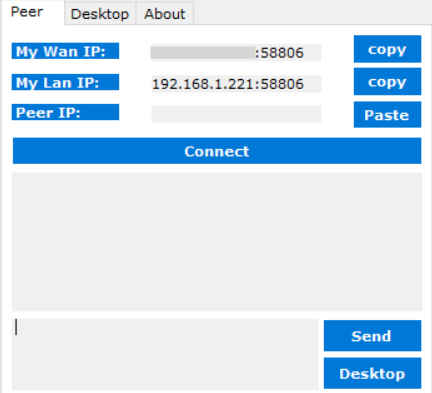
\includegraphics[width=15cm]{images/ui1.png}
	\caption{UI phase 1.1}
	\label{fig:form}
\end{figure}
\pagebreak
\begin{figure}
	\centering
	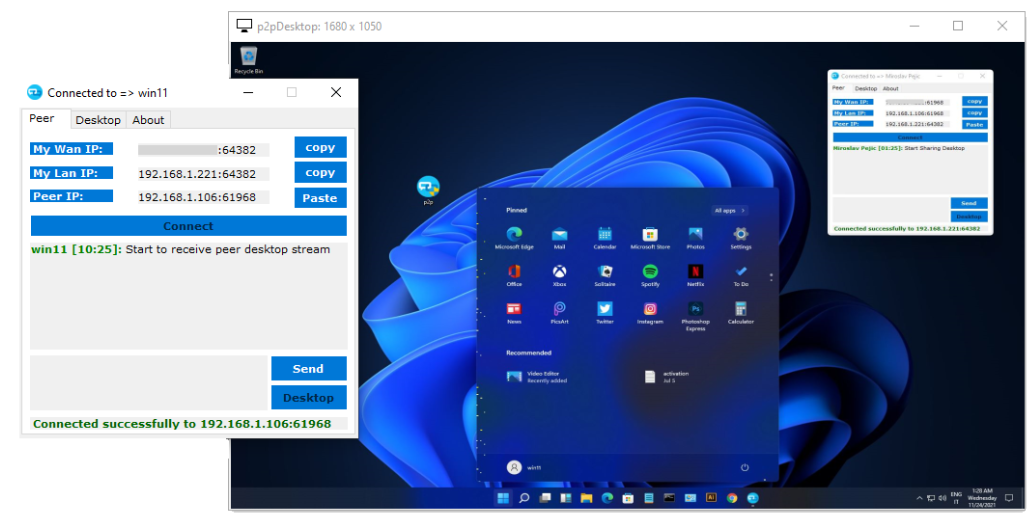
\includegraphics[width=15
	cm]{images/ui2.png}
	\caption{UI phase 1.2}
	\label{fig:form}
\end{figure}
\pagebreak
\section{Сервер}
Remote Web Browser хийх үйл явцыг эхний алхамаас нь сурахыг зорьсон бөгөөд файл болон чат Сервер хөгжүүлж үзсэн. 

Сурах ур чадвар: 
\begin{itemize}
    \item Админ эрхээр хэрхэн ажиллах
    \item CLI ажиллах
    \item Олон технологиудыг хооронд нь уяалдуулан ашиглах
\end{itemize}

Апп-ын шаардлага: 
\begin{itemize}
    \item Visual Studio ашиглах
    \item Тестын серверээс өгөгдөл татах
    \item Тестын сервер лүү өгөгдөл илгээх
\end{itemize}

\subsection{index.ts}
\begin{lstlisting}
	import Vue from 'vue'
	import Vuex from 'vuex'
	import { useAccessor, mutationTree, getterTree, actionTree } from 'typed-vuex'
	import { EVENT } from '~/neko/events'
	import { AdminLockResource } from '~/neko/messages'
	import { get, set } from '~/utils/localstorage'
	
	import * as video from './video'
	import * as chat from './chat'
	import * as files from './files'
	import * as remote from './remote'
	import * as user from './user'
	import * as settings from './settings'
	import * as client from './client'
	import * as emoji from './emoji'
	
	export const state = () => ({
		displayname: get<string>('displayname', ''),
		password: get<string>('password', ''),
		active: false,
		connecting: false,
		connected: false,
		locked: {} as Record<string, boolean>,
	})
	
	export const mutations = mutationTree(state, {
		setActive(state) {
			state.active = true
		},
	
		setLogin(state, { displayname, password }: { displayname: string; password: string }) {
			state.displayname = displayname
			state.password = password
		},
	
		setLocked(state, resource: string) {
			Vue.set(state.locked, resource, true)
		},
	
		setUnlocked(state, resource: string) {
			Vue.set(state.locked, resource, false)
		},
	
		setConnnecting(state) {
			state.connected = false
			state.connecting = true
		},
	
		setConnected(state, connected: boolean) {
			state.connected = connected
			state.connecting = false
			if (connected) {
				set('displayname', state.displayname)
				set('password', state.password)
			}
		},
	})
	
	export const getters = getterTree(state, {
		isLocked: (state) => (resource: AdminLockResource) => resource in state.locked && state.locked[resource],
	})
	
	export const actions = actionTree(
		{ state, getters, mutations },
		{
			initialise() {
				accessor.emoji.initialise()
				accessor.settings.initialise()
			},
	
			lock(_, resource: AdminLockResource) {
				if (!accessor.connected || !accessor.user.admin) {
					return
				}
	
				$client.sendMessage(EVENT.ADMIN.LOCK, { resource })
			},
	
			unlock(_, resource: AdminLockResource) {
				if (!accessor.connected || !accessor.user.admin) {
					return
				}
	
				$client.sendMessage(EVENT.ADMIN.UNLOCK, { resource })
			},
	
			toggleLock(_, resource: AdminLockResource) {
				if (accessor.isLocked(resource)) {
					accessor.unlock(resource)
				} else {
					accessor.lock(resource)
				}
			},
	
			login(store, { displayname, password }: { displayname: string; password: string }) {
				accessor.setLogin({ displayname, password })
				$client.login(password, displayname)
			},
	
			logout() {
				accessor.setLogin({ displayname: '', password: '' })
				set('displayname', '')
				set('password', '')
				$client.logout()
			},
		},
	)
	
	export const storePattern = {
		state,
		mutations,
		actions,
		getters,
		modules: { video, chat, files, user, remote, settings, client, emoji },
	}
	
	Vue.use(Vuex)
	
	const store = new Vuex.Store(storePattern)
	export const accessor = useAccessor(store, storePattern)
	
	Vue.prototype.$accessor = accessor
	
	declare module 'vue/types/vue' {
		interface Vue {
			$accessor: typeof accessor
		}
	}
	
	export default store
\end{lstlisting}
\pagebreak

\section{Клиент}

Веб хөтөч хийх үйл явцыг эхний алхмаас нь сурахыг зорьсон. 
\begin{figure}
	\centering
	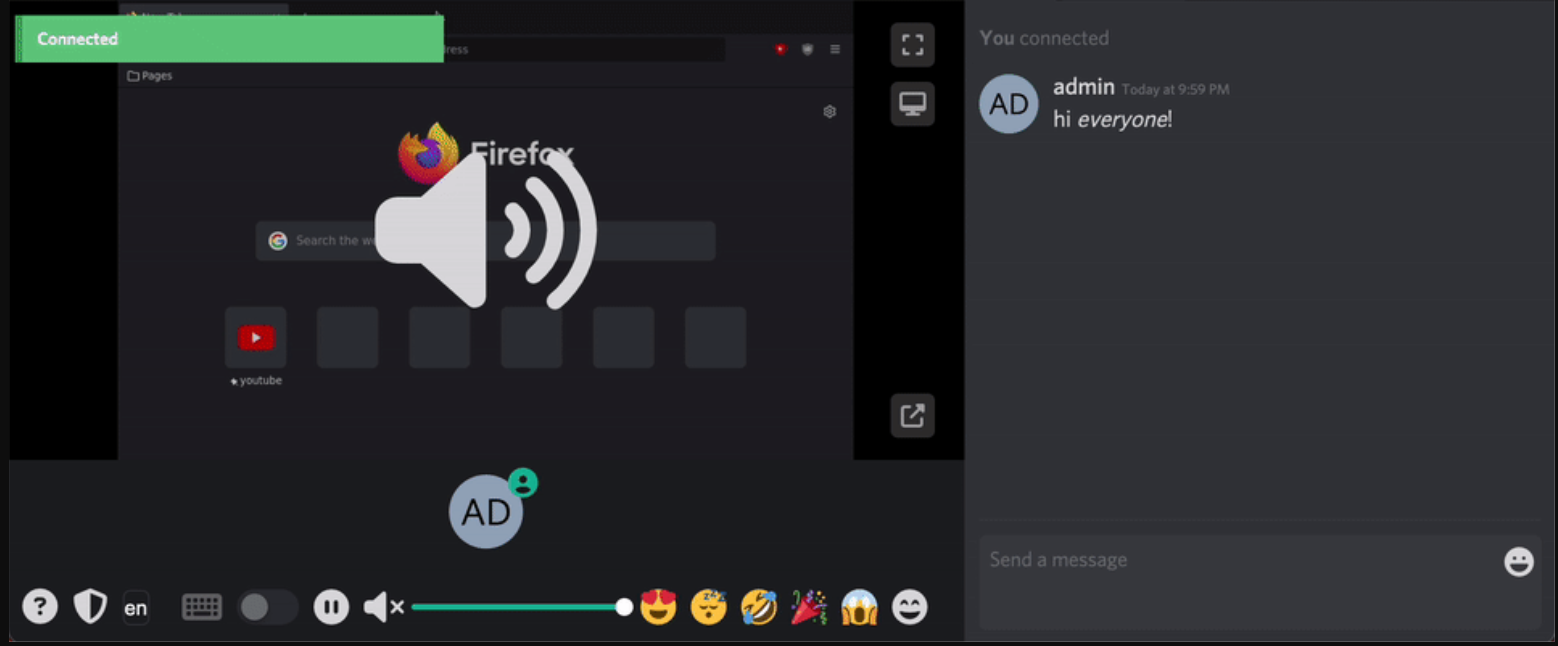
\includegraphics[width=15cm]{images/ui21.png}
	\caption{UI phase 2.1}
	\label{fig:form}
\end{figure}
\begin{figure}
	\centering
	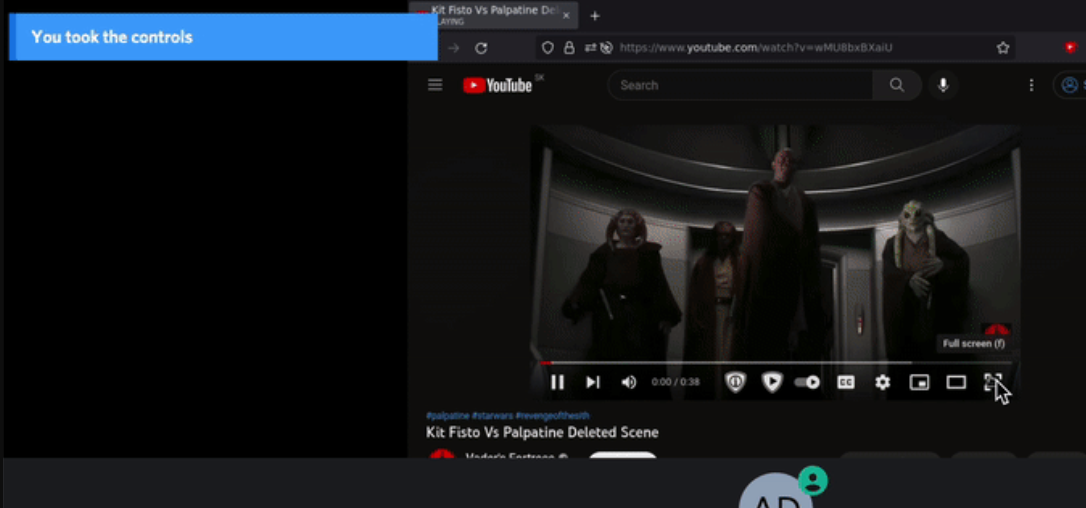
\includegraphics[width=15cm]{images/ui22.png}
	\caption{UI phase 2.2}
	\label{fig:form}
\end{figure}
Сурах ур чадвар: 
\begin{itemize}
    \item Алхам алхмаар нарийн сайн төлөвлөх
    \item Шинэ программыг хурдан сурах
    \item Minimalist design сурах
\end{itemize}

Апп-ын шаардлага: 
\begin{itemize}
    \item Visual Studio ашиглах
    \item Ямар ч ажлын байран дээр тохиромжтой байх
    \item Бүх насныхан ашиглахад тохиромжтой байх
\end{itemize}
\pagebreak
\subsection{Гол дэлгэцлэх хэсэг}
\begin{lstlisting}
	export function makeid(length: number) {
		let result = ''
		const characters = 'ABCDEFGHIJKLMNOPQRSTUVWXYZabcdefghijklmnopqrstuvwxyz0123456789'
		const charactersLength = characters.length
		for (let i = 0; i < length; i++) {
			result += characters.charAt(Math.floor(Math.random() * charactersLength))
		}
		return result
	}
	
	export function lockKeyboard() {
		if (navigator && navigator.keyboard) {
			navigator.keyboard.lock()
		}
	}
	
	export function unlockKeyboard() {
		if (navigator && navigator.keyboard) {
			navigator.keyboard.unlock()
		}
	}
	
	export function elementRequestFullscreen(el: HTMLElement) {
		if (typeof el.requestFullscreen === 'function') {
			el.requestFullscreen()
			//@ts-ignore
		} else if (typeof el.webkitRequestFullscreen === 'function') {
			//@ts-ignore
			el.webkitRequestFullscreen()
			//@ts-ignore
		} else if (typeof el.webkitEnterFullscreen === 'function') {
			//@ts-ignore
			el.webkitEnterFullscreen()
			//@ts-ignore
		} else if (typeof el.mozRequestFullScreen === 'function') {
			//@ts-ignore
			el.mozRequestFullScreen()
			//@ts-ignore
		} else if (typeof el.msRequestFullScreen === 'function') {
			//@ts-ignore
			el.msRequestFullScreen()
		} else {
			return false
		}
		return true
	}
	
	export function isFullscreen(): boolean {
		return (
			document.fullscreenElement ||
			//@ts-ignore
			document.msFullscreenElement ||
			//@ts-ignore
			document.mozFullScreenElement ||
			//@ts-ignore
			document.webkitFullscreenElement
		)
	}
	
	export function onFullscreenChange(el: HTMLElement, fn: () => void) {
		if (el.onfullscreenchange === null) {
			el.onfullscreenchange = fn
			//@ts-ignore
		} else if (el.onmsfullscreenchange === null) {
			//@ts-ignore
			el.onmsfullscreenchange = fn
			//@ts-ignore
		} else if (el.onmozfullscreenchange === null) {
			//@ts-ignore
			el.onmozfullscreenchange = fn
			//@ts-ignore
		} else if (el.onwebkitfullscreenchange === null) {
			//@ts-ignore
			el.onwebkitfullscreenchange = fn
		}
	}
\end{lstlisting}
\begin{figure}
	\centering
	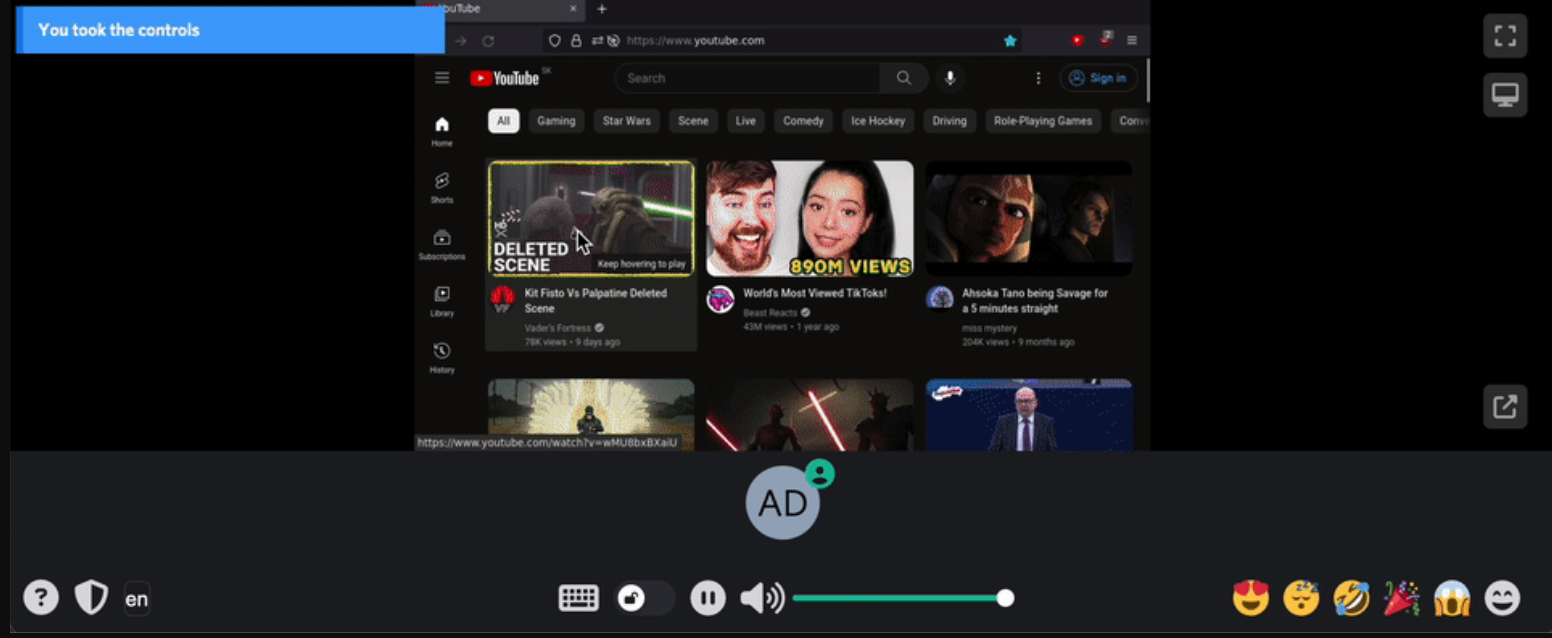
\includegraphics[width=15cm]{images/ui23.png}
	\caption{UI phase 2.3}
	\label{fig:form}
\end{figure}
\begin{figure}
	\centering
	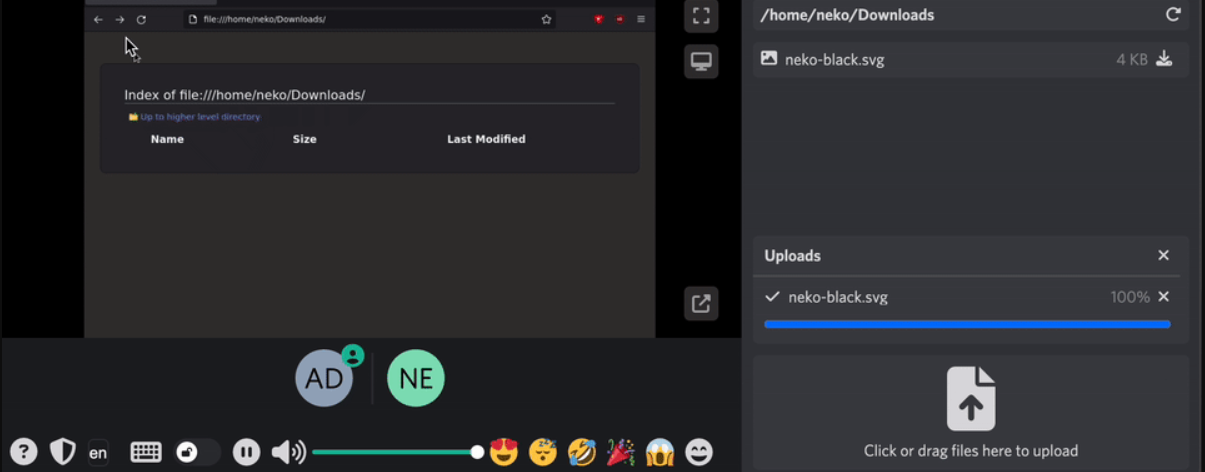
\includegraphics[width=15cm]{images/ui24.png}
	\caption{UI phase 2.4}
	\label{fig:form}
\end{figure}
